\documentclass{a0poster}
\usepackage{geometry}
%\geometry{paper=a1paper}
\geometry{width=630mm,height=594mm}
\geometry{hmarginratio=1:1}
\geometry{vmarginratio=1:1}
\geometry{hmargin=25mm}
\geometry{vmargin=25mm}
\usepackage[pdftex]{graphicx}
% \usepackage{curves}
% \usepackage{algorithmic}
\usepackage[utf8]{inputenc}
\usepackage{amsmath}
\usepackage{amssymb}
\usepackage{amsthm}
% \usepackage{color, graphicx}
\usepackage{lipsum}
\usepackage{multicol}
\usepackage{subfigure}
% \usepackage{textpos}
\usepackage{url}
\usepackage{xcolor}
\usepackage{rotating}

\usepackage{mathptmx}
\usepackage[scaled=.90]{helvet}
\usepackage{courier}

% paket från kex
% \usepackage[T1]{fontenc}
% \usepackage{textcomp}
% \usepackage{lmodern}
\usepackage[swedish, english]{babel} 
% \usepackage[pdftex]{graphicx}
% \usepackage{wrapfig}
% \usepackage{float}
% \usepackage{cite}
% \usepackage{subfigure}
%%% define new commands %%%

\DeclareMathOperator{\sgn}{sgn}
\DeclareMathOperator{\sign}{sign}
\DeclareMathOperator{\diag}{diag}
\DeclareMathOperator{\supp}{supp}
\DeclareMathOperator{\res}{res}
\DeclareMathOperator{\meas}{meas}

\def\tol{{\textsc{tol}}}
\providecommand{\D}[1]{\,\mathrm{d}#1}

%\newcommand{\mysmall}{\small}
%\newcommand{\mynormalsize}{\normalsize}
%\newcommand{\myFontSize}{\large}
%\newcommand{\myTitleFontSize}{\Large}
%\newcommand{\mySubTitleFontSize}{\large}
%\newcommand{\mySubSubTitleFontSize}{\small}
%\newcommand{\setLineThickness}{\linethickness{2mm}}
%\newcommand{\myrule}{\rule{\textwidth}{1pt}}

%%% set new tolerances %%%%

\renewcommand{\textfraction}{0.05}
\renewcommand{\topfraction}{0.95}
\renewcommand{\bottomfraction}{0.95}
\renewcommand{\floatpagefraction}{0.35}
\setcounter{totalnumber}{5}

%%% Set footnote numbering type %%%
\renewcommand{\thefootnote}{\arabic{footnote}}

%%% options for multcol
\setlength{\columnsep}{25mm}

%%% Graphics search paths %%%
\graphicspath{{figures/}{figures/hmm-graph/}{figures/gwhisker_database/}{figures/gwhiskers/}}

%%% Custom commands

\newcommand{\prob}[1]{p\left(#1\right)}
\newcommand{\cprob}[2]{\prob{\left. #1 \middle\vert #2 \right.}}
\newcommand{\cprobnext}[1]{\cprob{#1_{n+1}}{#1_n}}
\newcommand{\ndist}[2]{\mathcal{N}\left(#1, #2\right)}

%%% begin document %%%

\begin{document}

\begin{tabular}{ll}

  \begin{minipage}{630mm}

    {\Large\bf Probabilistic Tracking of Multiple Rodent Whiskers In Monocular Video Sequences}\\[3mm]
    {\bf Jim Holmström, \; Emil Lundberg\\
      Bachelor's Thesis at CSC, KTH} \\


    \vspace*{5mm}

  \end{minipage}

\end{tabular}

\vspace*{10mm}

\begin{minipage}{\linewidth}

  \begin{multicols*}{3}
    
    \section*{Background}
\subsection*{The Problem}
The interest in studying rodent whiskers has recently seen a significant increase, particularly in the field of neurophysiology. As a result, there is a need for automatic tracking of whisker movements. Currently available commercial solutions either are extremely expensive, restrict the experiment setup\footnote{A method known as \emph{optoelectronic monitoring} takes this to the extreme by having the rat locked in place by cranium-mounted screws \cite{Optoelectronic}. See figure \ref{fig:optoelectronic}.}, or fail in cluttered environments or when whiskers occlude each other. A cheap, reliable solution to the tracking problem is needed.

\begin{figure}[h]
  \centering
  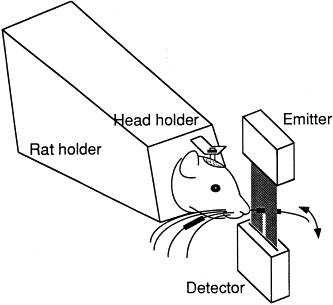
\includegraphics[width=0.3\textwidth]{optoelectronic.png}
  \caption{A very restrained experiment setup.}
  \label{fig:optoelectronic}
\end{figure}

\begin{figure}
  \centering
  \begin{tabular}{rl}
    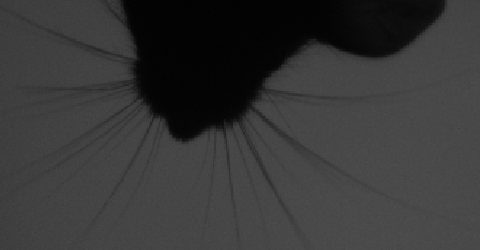
\includegraphics[width=0.5\textwidth]{rat-vanilla.png}
    & 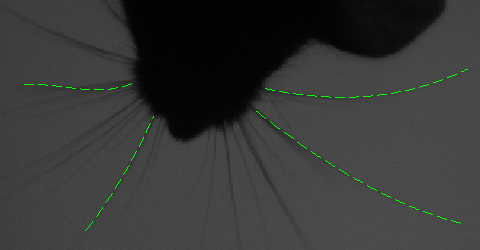
\includegraphics[width=0.5\textwidth]{rat-splines.png}
    \label{fig:rat}
  \end{tabular}

  \caption{Left: Example image of a rat and its whiskers. Right: Least squares fitted third degree polynomials.}
  \label{fig:whiskers}
\end{figure}

\subsection*{A Probabilistic Approach}
We propose solving the problem by a probabilistic approach. We use a technique known as the \emph{Particle Filter} to propagate a whisker model between frames of high speed video. In each frame, the next state of the model is predicted by searching a pre-trained database, and filtering the results through the Particle Filter. The main difference between this and existing solutions is that it maintains a model of the whiskers. This makes it easier to keep track of them even when they cross or overlap.

    
    \section*{The Probabilistic Framework}
Our solution is based on \emph{Markov processes}, which are a special case of stochastic processes. For a Markov process, the next state depends only on the present state and not on past states.

An example of a Markov process is that of throwing dice and summing the results: the possible states (sums) after the next throw depend only on the current state, and not on the results of the individual throws.

In mathematical terms, a Markov process satisfies the following:
\begin{equation}
 \cprob{Z_{n+1}}{Z_n \wedge Z_{n-1} \wedge \dots \wedge Z_0} = \cprob{Z_{n+1}}{Z_n}
\end{equation}
where $Z_n$ is the system's \emph{state} after step $n$ and $\cprob{Z_{n+1}}{Z_n \wedge Z_{n-1} \wedge \dots \wedge Z_0}$ is the probability that the system will have state $Z_{n+1}$ in the next step, given that the previous states were $Z_n, Z_{n-1}, Z_{n-2}, \dots, Z_0$.

A \emph{hidden Markov model} (HMM) describes a Markov process where one cannot measure the state $Z$ of the system directly - it is ``hidden'' - but rather obtains an \emph{observation} $I$\footnote{In this project, the observation is a grayscale \emph{image}, which is why we use the symbol $I$.}  of the state by some \emph{perception}. The observation is generally non-deterministic, so we need to denote it as $p(I_n|Z_n)$ which is the probability that we will observe $I_n$ if the current state of the system is $Z_n$.

\subsection*{The Particle Filter}
The Particle Filter is a technique for simulating a process described by a HMM. It uses a finite set $X_n$ of $N$ hypotheses to approximate the probability function $p(Z_n)$ above. The hypotheses $X_n$ are also known as \emph{particles}, thereby the term ``particle filter''. In short terms, the particle filter does the following:

\begin{enumerate}
  \item Predicts the next state $Z_{n+1}$ by drawing samples $X_{n+1}$ from $p(Z_{n+1} | Z_n)$,
  \item resamples the hypotheses $X_{n+1}$ by drawing new samples from $p\left(I_{n+1} | x_{n+1}^i\right)$
\end{enumerate}


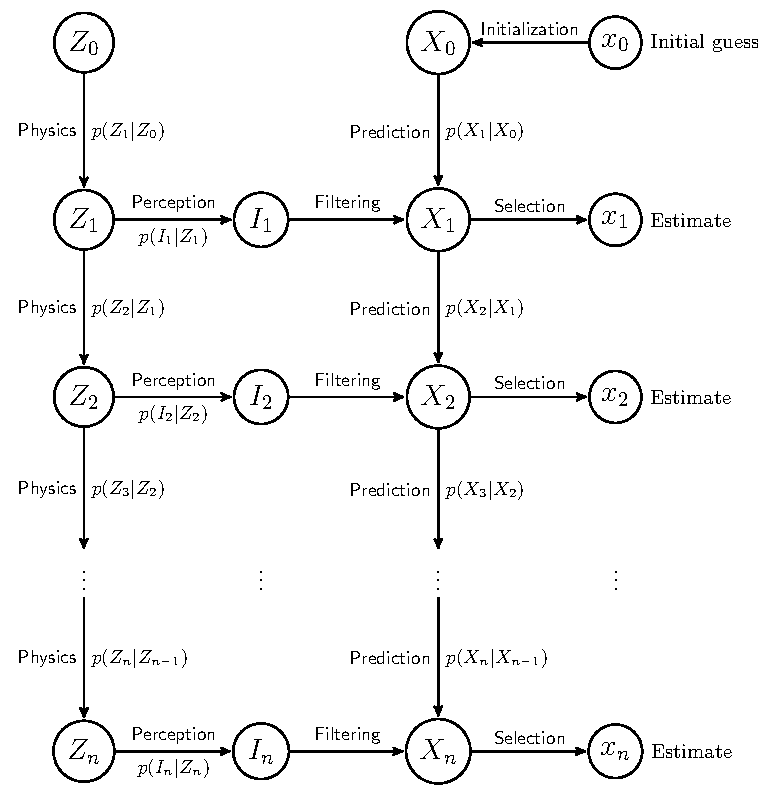
\includegraphics[width=0.3\textwidth]{figures/hmm-graph/hmm-graph.pdf}
Above is an illustration of a Particle Filter working with a Hidden Markov Model. The system assumes states $Z_0, Z_1, ...$ with probabilities $p(Z_0), p(Z_1|Z_0), \cdots$, and we obtain the observations $I_1, I_2, \cdots$ with probabilities $p(I_1|Z_1), p(I_2|Z_2), \cdots$. Parallel to this, we have a set of hypotheses $X$ for the state $Z$. The hypotheses $X_n$ of $Z_n$ are updated in the \emph{prediction} step to hypotheses $\bar{X}_{n+1}$ of $Z_{n+1}$. The image $I_{n+1}$ of the system is then used in the \emph{resampling step} to select the best hypotheses from $\bar{X}_{n+1}$, yielding the \emph{belief} $X_{n+1}$. Finally, we create a single hypothesis $x_{n+1}$ from $X_{n+1}$ that will be our estimate of the state $Z_{n+1}$.


    \section*{Our implementation of the Particle Filter}
An implementation of the Particle Filter consists mainly of designing the probability functions $\cprobnext{X}$ and $\cprob{I_n}{X_n}$, and providing the algorithm with a sensible initialization. This is what this project is all about. The rest just consists of taking samples from these functions.

\subsection*{The prediction step: The Database}

We investigate the plausibility of implementing $\cprobnext{X}$ as a search through a database of training data. We set up a database of known transitions between whisker shapes. A transition $T$ consists of a ``from'' state $f$ and a''to'' state $t$. This denotes our \emph{ground truth}\footnote{See \cite{EncyclopediaMachineLearning}} that ``a whisker went from this shape to that shape in one time step''. We then approximate $\cprobnext{X}$ as a weighted average of the database, where transitions are weighted by how much their ``from'' parts differ from the hypotheses in $X_n$.

What we do in practice when sampling is: for each hypothesis $x_n^i \in X_n$,

\begin{enumerate}
  \item For each transition $T^j = (f^j, t^j)$ in the database, calculate the function $d^{ij}$ that is the difference between the two functions described by $x_n^i$ and $f^j$. In this case, both are polynomials and thus $d^{ij}$ is the polynomial with coefficients given by the tuple $x_n^i - f^j$.
  \item Let $w^{ij} = \left(\frac{1}{\norm{d^{ij}}_{\Lp{p}}}\right)^a$, the reciprocal of the $\Lp{p}$ norm of $d^{ij}$ raised to a power $a$.
  \item Return $\frac{\sum_j t^j w^{ij}}{\sum_jw^{ij}}$, the weighted average of the ``to'' states with weights $w^{ij}$.
\end{enumerate}

Doing this for each hypothesis $x_n^i$ yields the set $\bar{X}_n$.

We have not yet thoroughly investigated which power $a$ and which $\Lp{p}$ space to use. We have run tests with $\Lp{2}$, and $a=4$ seems to be a good value. These will later be determined in a ``bake-off''\footnote{See \cite{EncyclopediaMachineLearning}}.

\subsection*{The filtering step: Image comparison}

\begin{figure}
  \centering
  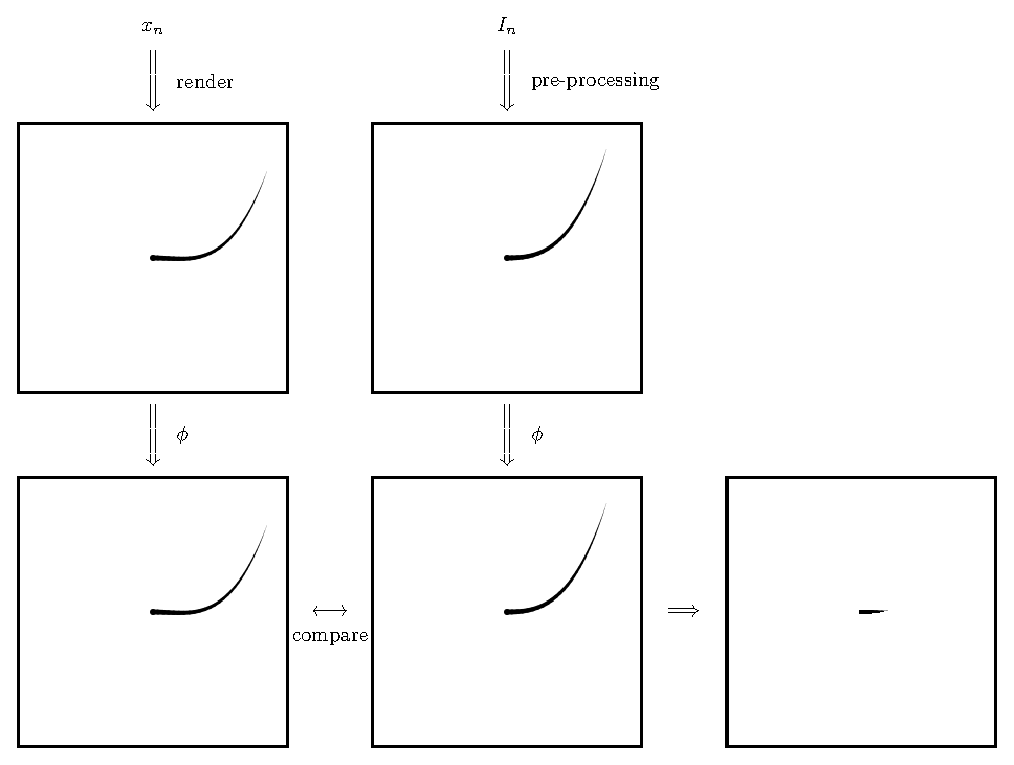
\includegraphics[scale=1.0]{whisker_compare.pdf}
  \caption{Schematic image of the process to evaluate the importance of a hypothesis. The transformation $\phi$ in this case extracts an edge cue from the images.}
  \label{fig:whisker_compare}
\end{figure}

We implement the probability function $\cprob{I_n}{X_n}$ as a comparison between $I_n$ and the images corresponding to the hypotheses $X_n$. For each hypothesis $\bar{x}_n^i \in \bar{X}_n$ we create an image $I_n^i$ that corresponds to the state described by $\bar{x}_n^i$.

We apply a transformation $\phi$ to the images to get a sensory cue for evaluating the hypotheses. At the current stage in our testing, the images used are generated synthetic ones that are already easy to process. Therefore we let $\phi$ be the identity transformation at the moment. Another feasible candidate for $\phi$ would be a differentiation, in order to highlight edges in the image.

We then let $w^i = \sum\limits_{\mathrm{pixels}}\phi\left(I_n\right) \cdot \phi\left(I_n^i\right)$, where the multiplication is done component-wise. We then let $\left\{\left(\bar{x}_n^i, w^i\right)\right\}_{i=1}^N$ define a discrete probability function that returns $\bar{x}_n^i$ with probability $\frac{w^i}{\sum_{i=0}^Nw^i}$, and let this distribution be our approximation of $\cprob{I_N}{X_n}$.

\begin{figure}
  \centering
  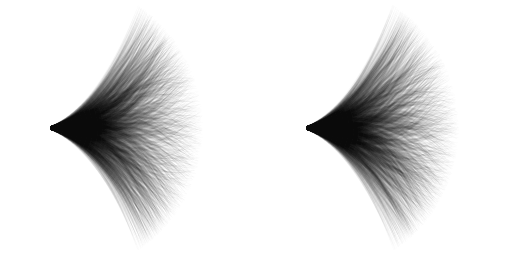
\includegraphics[width=0.7\textwidth]{database_gwhisker_spline3_n2048_from_to_fixed.png}
  \caption{View of all whiskers in transition database. Left: from-states. Right: to-states.}
  \label{fig:database}
\end{figure}

\subsection*{Example tracking image}

Figure \ref{fig:particles} shows an illustration of the three tracking steps. The blue lines are the hypotheses $\bar{X}_n$ sampled from the database. The red lines are these same hypotheses, but after resampling, $X_n$. The green line is the estimate $x_n$, the mean of $X_n$. One can see how $X_n$ is slightly more concentrated around the tracked whisker (white) than $\bar{X}_n$ is.

\begin{figure}[h]
  \centering
  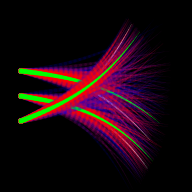
\includegraphics[width=0.3\textwidth]{tracking-particles.png}
  \caption{Tracking image with $\bar{X}_n$ (blue) and $X_n$ (blue) drawn along with the estimate $x_n$ (green).}
  \label{fig:particles}
\end{figure}


    
    
The bake-off <ref> setup:

Evaluated parameters:
    p     - for the norm
    a     - penelty for the norm
    N     - number of transitions
    cp    - particle count
    sigma - on resample blur

will be tested on a small set of benchmarks consisting of 4 disperse(d?)/scatter generated whisker videos.

The test matrix:
\begin{equation}
    \Phi_{p,a,N,...}(benchmark)
\end{equation}

The measures we will use as fitness of the algorithm is:
    integrating over time the the difference with the ground truth (do this for L{1:10} and see if it correlates with the p choosed
    integrating over time the response for the choosed hypotethis (to see how the image transformation affects the results)
    4 image samples (checked by hand, subjective)


"There are many metrics by which a model may be assessed." - Encyclopedia
(>model evaluation)

"A learning algorithm must interpolate appropriate predictions for regions of
the instance space that are not included in the training data." - Encyclopedia
(>model evaluation)

<<graph over the setup>>

The fitness test was runned on different machines but this wont effect the
result since we initially wont consider the running time.

The runtime for the algorithm is handled separately on one machine setup <...>




(performance vs fitness)

** Theoretical evalutaion (formal methods)
** Experimental algorithm evaluation 


"
However, much machine learning
research includes experimental studies in which algo-
rithms are compared using a set of data sets with little
or no consideration given to what class of applications
those data sets might represent. It is dangerous to draw
general conclusions about relative performance on any
application from relative performance on this sample
of some unknown class of applications. Such experi-
mental evaluation has become known disparagingly as
a bake-off .
" - Encyclopedia (>algorithm evaluation)



Can a particlefilter overfit?


>Hypothesis space (

"
==Model selection
Model selection is the process of choosing an appropriate mathematical model
from a class of models.
" - Encyclopedia 
The class being all functions with f(0)=0,contioiuns(stronger?) and finite number of parameters




    \section*{The Database}

\begin{center}
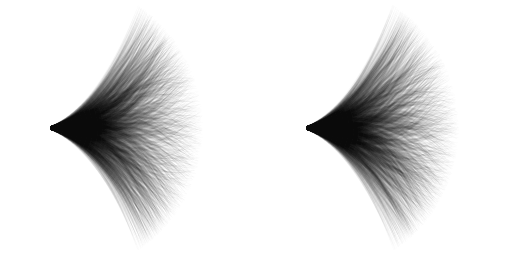
\includegraphics[scale=1.0]{database_gwhisker_spline3_n2048_from_to_fixed.png}
\label{fig:database}

Figure 3: View of all whiskers in transition database, from-states on the left and to-states on the right.
\end{center}

    \section*{A Simple Whisker Model}

Our simplest model of a whiskers is $n$-th degree polynomial curve attached at $x=0$ to a fixed point in space. This means our state parameters are the coefficients ${a_i}_{i=0}^n$ of the polynomial $\sum_{i=0}^n a_ix^i$. In this model we implicitly assume that the rat's head movements do not greatly affect the whiskers' movement. Possible improvements to this model may include:
\begin{itemize}
  \item letting the whisker attach to a fixed point in a moving coordinate system (the ``head system''),
  \item using some other function basis, such as a sine series.
\end{itemize}

So far we have only investigated the simplest polynomial model. Least squares fitting tests performed using MATLAB show that a third degree polynomial can represent any whisker in Figure 1 with an error that is not visible to the naked eye. Therefore a third degree polynomial was used. We omit the constant term since this information can instead be included in the position of the whisker base.

\begin{center}
  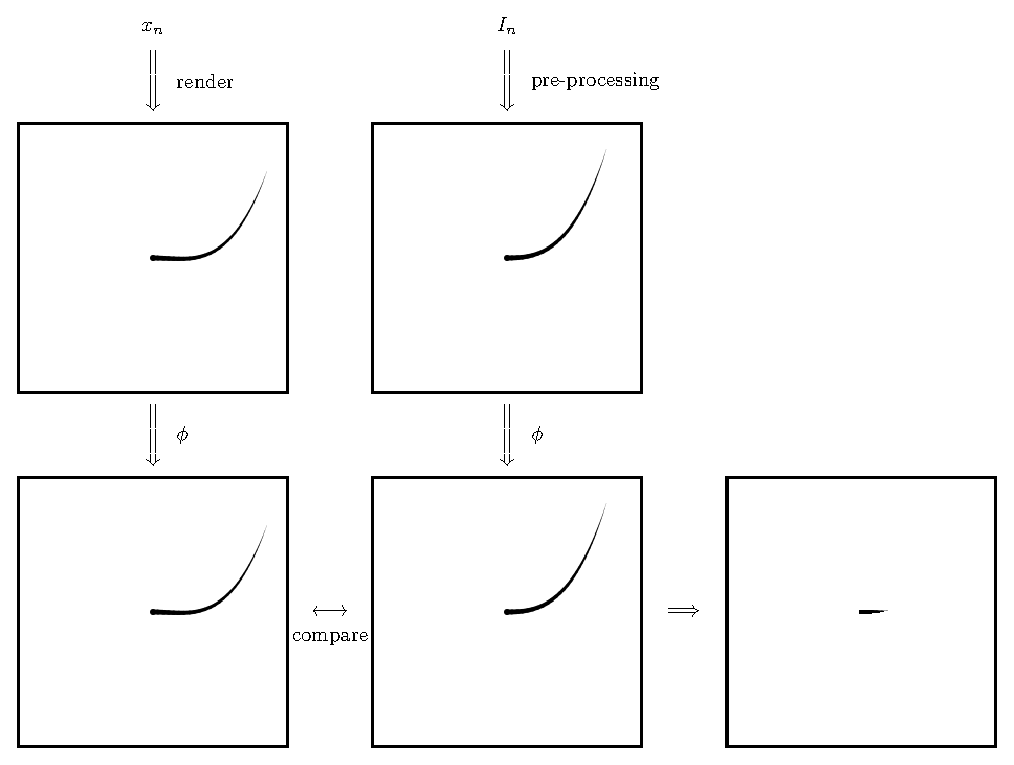
\includegraphics[scale=1.5]{whisker_compare.pdf}
\end{center}



    \bibliographystyle{vancouver}
    \bibliography{a0poster}

  \end{multicols*}

\end{minipage}


\end{document}
